%% $RCSfile: proj_report_outline.tex,v $
%% $Revision: 1.3 $
%% $Date: 2016/06/10 03:41:54 $
%% $Author: kevin $

\documentclass[11pt
              , a4paper
              , twoside
              , openright
              ]{report}


\usepackage{float} % lets you have non-floating floats
\usepackage{threeparttable}
\usepackage{url} % for typesetting urls
\usepackage{listings} % needed for the inclusion of source code
\usepackage{color}
\usepackage{caption}
\usepackage[toc]{appendix}
\usepackage{graphicx}
\usepackage{epigraph}
\usepackage{amsmath}
\usepackage{subcaption}


\graphicspath{ {/images/} }

\definecolor{dkgreen}{rgb}{0,0.6,0}
\definecolor{gray}{rgb}{0.5,0.5,0.5}
\definecolor{mauve}{rgb}{0.58,0,0.82}

\lstset{frame=tb,
  language=Java,
  aboveskip=3mm,
  belowskip=3mm,
  showstringspaces=false,
  columns=flexible,
  basicstyle={\small\ttfamily},
  numbers=none,
  numberstyle=\tiny\color{gray},
  keywordstyle=\color{blue},
  commentstyle=\color{dkgreen},
  stringstyle=\color{mauve},
  breaklines=true,
  breakatwhitespace=true,
  tabsize=3
}

\lstnewenvironment{42listing}
    {
\lstdefinelanguage{L42}{
  keywords={assert, for, while, switch, if, case, return, with
    else, in, mut, <><, reuse, import, Void,  Library, Refactor
   bool, in, var, method, class, Num, Collections, interface, implements, extends
  },
  keywordstyle=\color{blue},
  basicstyle=\ttfamily,
  numbers=none,
  numberstyle=\tiny\color{gray},
  commentstyle=\color{dkgreen},
  stringstyle=\small\itshape,
  moredelim=*[s][commentstyle]{/*}{*/}, 
  morecomment=[l][commentstyle]{//}      
}
\lstset{
        language = L42,
        basicstyle=\ttfamily,
        breaklines=true,
        columns=fullflexible}
	}
{}



%
%  We don't want figures to float so we define
%
\newfloat{fig}{thp}{lof}[chapter]
\floatname{fig}{Figure}

%% These are standard LaTeX definitions for the document
%%                            
\title{Debugging the 42 Prototype}
\author{Aden Kenny}

%% This file can be used for creating a wide range of reports
%%  across various Schools
%%
%% Set up some things, mostly for the front page, for your specific document
%
% Current options are:
% [ecs|msor|sms]          Which school you are in.
%                         (msor option retained for reproducing old data)
% [bschonscomp|mcompsci]  Which degree you are doing
%                          You can also specify any other degree by name
%                          (see below)
% [font|image]            Use a font or an image for the VUW logo
%                          The font option will only work on ECS systems
%
\usepackage[image,ecs]{vuwproject}

% You should specifiy your supervisor here with
%     \supervisor{Firstname Lastname}
% use \supervisors if there is more than one supervisor

\supervisor{Dr. Marco Servetto}

% Unless you've used the bschonscomp or mcompsci
%  options above use
%   \otherdegree{OTHER DEGREE OR DIPLOMA NAME}
% here to specify degree

\otherdegree{Bachelor of Engineering with Honours}

% Comment this out if you want the date printed.
\date{}

\begin{document}

% Make the page numbering roman, until after the contents, etc.
\frontmatter

%%%%%%%%%%%%%%%%%%%%%%%%%%%%%%%%%%%%%%%%%%%%%%%%%%%%%%%

%%%%%%%%%%%%%%%%%%%%%%%%%%%%%%%%%%%%%%%%%%%%%%%%%%%%%%%

\begin{abstract}
~\\
42 is a statically typed, high-level programming language developed by Dr. Marco Servetto at Victoria University of Wellington. The 42 compiler, like the vast majority of software systems, is not bug-free. This project focused on the creation of 42 programs to find previously unknown bugs in the compiler. A black-box testing methodology was employed to create these programs. This project has produced numerous tests that have identified thirty-two previously unknown bugs in the 42 compiler.


\end{abstract}

%%%%%%%%%%%%%%%%%%%%%%%%%%%%%%%%%%%%%%%%%%%%%%%%%%%%%%%

\maketitle

\chapter*{Acknowledgments}\label{C:ack} 

I wish to thank my supervisor, Dr. Marco Servetto, for his help and guidance throughout this project. I also wish to thank Cas for proofreading this report, and making me coffee when I needed it most.

\tableofcontents

% we want a list of the figures we defined
\listof{fig}{Figures}

%%%%%%%%%%%%%%%%%%%%%%%%%%%%%%%%%%%%%%%%%%%%%%%%%%%%%%%

\mainmatter

%%%%%%%%%%%%%%%%%%%%%%%%%%%%%%%%%%%%%%%%%%%%%%%%%%%%%%%

% individual chapters included here
\chapter{Introduction}\label{C:intro}

\makeatletter
\renewcommand{\@chapapp}{}% Not necessary...
\newenvironment{chapquote}[2][2em]
  {\setlength{\@tempdima}{#1}%
   \def\chapquote@author{#2}%
   \parshape 1 \@tempdima \dimexpr\textwidth-2\@tempdima\relax%
   \itshape}
  {\par\normalfont\hfill--\ \chapquote@author\hspace*{\@tempdima}\par\bigskip}
\makeatother

42 is a statically typed, high-level programming language designed to allow the use and composition of millions libraries simultaneously \cite{L42}. The current implementation of 42 is written in Java. The 42 compiler is a large and complex piece of software which consists of over 70,000 lines of code. It is highly likely that bugs exist in the implementation of practically any language \cite{arnabold}, and the main way to find these bugs is through testing. Compiler bugs present a major problem as in the worst case scenario they can introduce bugs into previously bug-free code when it is compiled; causing the and programmer to spend a significant amount of time and effort attempting to track down the bug in their own code, rather than in the compiler. Compiler-introduced bugs are considered to be extremely difficult to find and track down \cite{Leroy:2009}. It is therefore important to locate bugs that exist in a compiler.

The goal of this project was to create programs that would try "to leverage corner cases of the implementation and discover bugs" \cite{outline}. From this it was decided that the main focus of this project was the designing, writing, compiling, and running of short programs. These programs were then converted into automated tests, minimised, and added to the 42 test suite. A black-box testing methodology \cite{ostrand} was chosen for this project to develop tests as the gathered requirements indicated that the system as whole should be tested. This strongly suggested a black-box approach should be taken. Alternative testing methodologies were considered for this project, but for various reasons these alternative approaches were found to be inadequate, inferior to the chosen approach, or not suited to the requirements of the project. These alternative approaches included a white-box testing methodology, or a more automated, fuzzing focused methodology.
 

\section{Contributions}

The contributions of this project are:

\begin{enumerate}
	\item{The creation of numerous 42 programs that were turned into automated tests.}
	\item{A reduction in the number of unknown bugs in the 42 compiler.}
	\item{A tool to turn 42 programs into automated tests.}
\end{enumerate}
\chapter{Background and Related Work} \label{C:background}

\section{Compiler Correctness}
A compiler is an extremely large and complex piece of software. As such, it is highly likely that bugs exist in the implementation of practically any language \cite{arnabold} and 42 is no exception to this. Complier testing can be a difficult and time consuming process and Leroy \cite{Leroy:2009} states that compiler-introduced bugs are widely considered to be extremely difficult to find and track down. In this section we will explore some of the current approaches to compiler testing that are considered most important to this project.

\subsection{CompCert}
One of the best ways to truly prove a non-trivial software system is bug free is through formal verification and Miller \cite{Miller:1990} states that the best way to make a systematic statement about the correctness of the code is to use formal methods, but the work required to create a formally verified complier of any real scale is a major barrier to using formal methods in compilers. The only example of a large scale compiler being fully formally verified is CompCert as presented by
Leroy \cite{Leroy:2009}. CompCert is a formally verified compiler for a large subset of the C language \cite{Blazy:2006} \cite{Blazy:2009}. CompCert is a verified compiler that provides some semantic preservation and has
"a mathematical, machine-checked proof that the generated executable code behaves exactly as prescribed by the semantics of the source program" \cite{CompCert}.This, theoretically, rules out the possibility of bugs being introduced by the compiler and means that any bug free code that is compiled will produce a bug free program.

The CompCert compiler is an interesting project, but to carry out a similar project for the 42 language is unrealistic for multiple reasons. First and foremost is that the writing of a formally verified compiler is significantly out of scope of this project, especially considering the CompCert compiler has had over six man-years of effort spent on it. Additionally if the approach used by Leroy was to be applied to a language different to the C subset introduced by Blazy \cite{Blazy:2009} some issues may arise. These issues would relate to verifying some 42 language features such as metaprogramming that could be difficult to verify.


\section{Automated Testing}
\subsection{Fuzzing}
Fuzzing is the technique of supplying random input into a program or application. This technique is quite often considered to be quite simple \cite{Miller:1995} but can be effective as it is fairly easy to implement, especially if existing tools can be used, and can find a large number of bugs\cite{Miller:1990} \cite{Miller:1995} \cite{Miller:2000} \cite{arnabold}. An example of a modern, well used fuzzing tool is \textit{american fuzzy lop} (AFL) \cite{afl}. AFL differs from other older and less advanced fuzzing tools such as \textit{fuzz} \cite{Miller:1990} by the use of compile-time instrumentation and genetic algorithms. This allows AFL to "discover clean, interesting test cases that trigger new internal states in the targeted binary" \cite{afl}. AFL has been used to find bugs in major programs such as \textit{Apple Safari}, \textit{llvm}, \textit{Adobe Reader}, and \textit{VLC} \cite{afl}.

\subsubsection{Potential Fuzzer Usage}
A potential issue with using AFL is that the interface to run it on Java programs \cite{javaAfl} is less used, and less well documented than the standard AFL version.
While fuzzers are a useful tool that have worked well on similar projects such as \textit{llvm}, using a fuzzer on the 42 compiler may present some issues. Perhaps the most problematic issue would be compilation time of a 42 program using the 42 compiler. Compiling a 42 program currently takes a significant period of time if the full standard library is used (around 30 seconds on fairly standard consumer hardware), and when large numbers of programs are compiled, the time taken would quickly add up. Additionally a fuzzer would probably have to be written to properly test 42, and it would have to be quite advanced to provide any meaningful results. If a fuzzer were to be used it would probably not be particularly effective unless significant amounts of time were spent writing it.

\section{General Testing Literature}
\subsection{Compiler Testing}

Unfortunately, literature on compiler testing is scarce \cite{jai}, but this section will briefly discuss some of the papers that do exist in this body of literature.

\subsubsection{Automated Testing}
In a paper presented by Chen et al. the topic of automated compiler testing is introduced \cite{Chen:2017}. They note that traditional automated testing techniques such as fuzzing have performance issues; with many tests and a significant amount of time needed to find bugs. They then introduce the concept of "learning to test" and propose LET, an approach to compiler testing that allows the prioritisation of test programs through a learning process, where a model is trained. This model is then used to prioritise test programs based on their likelihood of finding a bug and their performance costs. The results are quite impressive with around 60\% of test cases being sped up by at least 25\%. While the results are significant, the usage of these findings in regards to the test of the 42 compiler seems unlikely. This is primarily due to the approach being cutting edge, and seemingly difficult and time consuming to replicate or use, event if it were to be available.

In another paper, Chen et al. present a comparison of automated compiler testing techniques \cite{Chen:2016}. They compare three different techniques, Randomized Differential Testing (RDT), Different Optimization Levels (DOL) (a variation of RDT), and Equivalence Modulo Inputs (EMI). The results show that DOL is effective at finding bugs relating to optimisation, and RDT is generally more effective at detecting other types of bugs, but all three techniques can be used in conjunction with one anothe and complement each other. The results presented here are not particularly useful to this project as 42 does not have a heavily optimising compiler or different levels of optimisation, therefore DOL would not be of much use if applied to this project. RDT is used with two different compilers implementing the same specification and 42 only has a single compiler implementation therefore RDT would also not be very useful for this project.

Kossatchev and Posypkin present a survey of "Compiler Testing Methods" \cite{Kossatchev}. A key idea that can be taken from this paper is that "the algorithms for generating syntax-oriented test suites are time-tested ones. There remains a question of whether the use of automated methods for generating semantics-oriented tests ...  is justified from the practical standpoint, since the approaches discussed have been tested on subsets of real languages or on model programming languages". This can be related to 42, where it is clear that automated methods of generating simple programs that test the syntax of the language is a fairly easy task. In contrast it is likely that automated testing of non-syntax, or more "semantic-orientated" parts of the language would be significantly harder. This is due to the fact that it could potentially require the automated tool to "learn" how to generate 42 programs that are valid and complex enough to test anything beyond the parser. This paper raises some doubts over the usefulness of automated compiler testing for this project, especially in regards to the use of fuzzers as discussed previously. It is felt that any fuzzer used on, or created for this project is unlikely to find many bugs.  

 Additionally, the 42 parser was created with ANTLR \cite{antlr}. This means that any bugs that relate to the 42 parser would most likely be ANTLR bugs, which while being significant and definitely worthy of attention, are not the focus of this project.
While it is certainly possible that bugs exist in the 42 parser, and it is known that parsing bugs can be extremely serious, especially from a security perspective \cite{parserBugs}, we feel that testing of other language features such as the type system and syntax are of a higher priority at the present  time.

The development of an automated testing tool is often a significant effort, and generally requires significant amounts of development time and expertise \cite{enc2}. Test automation done well is a long term investment rather than a shortcut to better or cheaper testing \cite{enc2}. Fewster and Graham note that it is generally during the later maintenance of the system, rather than during the development process, that the benefit that automated testing tools provide start to outweigh the development costs \cite{sta}.

\subsection{Traditional Testing}

\subsubsection{Black-box Testing}
Ostrand defines black-box testing as "any method of generating testcases that is independent of the software's internal structure" \cite{ostrand}. Nidhra \cite{nidhra} states that "the main advantage" of black-box testing is that a tester is not required to have knowledge of the programming language a system is implemented in, nor knowledge of the system itself. Nidhra also states that black-box testing aids "in overall functionality validation of the system" \cite{nidhra}. This is important for a compiler as it would prove difficult to have complete knowledge of the overall system of a non-trivial compiler. Therefore, in the case of black-box testing a compiler, a tester would not have to have specific knowledge of the compiler or the source code. They would construct programs and attempt to compile them with the compiler that is being tested. The tester would then compare the expected output of running the compiled code with the actual output, and if the actual output differs from the expected output, a bug has been identified. An issue that must be kept in mind with this style of testing on a compiler is that it is reasonable that the tester will write code that is incorrect, and if the tester does not realise this, it is possible that an identified bug is a false positive.

When black-box testing, the tester should consider the purpose of the program, the possible inputs and outputs, the possible ways the program may fail, and the potential uses of the program \cite{ostrand}. 

A fairly common type of black-box testing is model-based testing, where the tester will create a model of "the process that the software is supposed to carry out" \cite{ostrand}. Finite-state machines are commonly used for modelling state-based and interactive systems. Model based testing can be difficult and complex when attempting to test large and complex systems, as it can be difficult to capture the entirety of the behaviour of the system in the model.

Another major type of black-box testing is use case testing \cite{ostrand}. For use case testing, test cases are constructed from descriptions of how the system should work or process tasks or events. A scenario is created with preconditions that must hold before the scenario takes place, and with postconditions that must hold after the scenario takes place. When the test is run, the outputs are compared against the postconditions for correctness, and if the outputs match postconditions the test has succeeded.

\subsubsection{White-box Testing \label{whitebox}}
Ostrand defines white-box testing as "test methods that rely on the internal structure of the software" \cite{ostrand}. White-box testing methods are designed to cover specific elements of the code by testing that specific element. The ideal case for white-box testing is to "test every part of the code in every way that it could be executed during actual operation of the system"  \cite{enc2}. Unfortunately, this ideal case is only possible in very simple programs with finite input domains \cite{enc2}. In practice, white-box test methods are generally used for checking the effectiveness and adequacy of black-box testing methods \cite{enc2}. At the end of the testing cycle white-box methods are sometimes employed to create tests to fill in the gaps of black-box testing \cite{ostrand}. 

Types of white-box testing methods include statement coverage testing, in which every single statement in the program is executed and checked to make sure the result is correct \cite{enc2}. This results in very thorough coverage of the program but may not take into account different paths that the program may have taken to get to a specific statement. Taking different paths through the program may result in different behaviour.

 Branch coverage testing is similar to statement coverage; however rather than every statement being tested, every possible branch that could be taken in the program is taken and therefore tested. Branch coverage is generally considered to be the bare minimum for a program to be considered thoroughly tested in a white-box methodology \cite{enc2}.

White-box testing often takes the form of unit testing, where the program is tested component by component. A component in this case, is the smallest possible testable part of the program. The smaller and simpler the component, the easier it is to test. 

Marciniak states that a common belief is that test suites with a high branch or path coverage will find a substantial number of bugs, but he states that "this has not been verified with controlled studies of real software" \cite {enc2}.

White-box testing presents the advantage of  being able to expose implementation errors that do not have anything to do with the problem specification. This means that white-box tests may catch bugs that would not be considered when purely thinking in terms of the program specific \cite{enc2}. Additionally, white-box testing has a natural concept of how much of the program is actually tested, through statement and branch coverage statistics.

A white-box testing methodology does present some disadvantages, Marciniak notes that "exercising a particular faulty statement or branch is no guarantee that the test input used is one that actually causes a failure to occur" \cite{enc2}.

\subsubsection{Grey-box testing}

Grey-box testing is the combination of white-box and black-box testing. It attempts to combine the advantages of both white-box and black-box testing while minimising the disadvantages of both \cite{ostrand}.

 Generally, when black-box testing, the tester has no knowledge of the internal nature of the system, and when white-box testing, the tester has complete knowledge of the internal nature and implementation of the system. A grey-box tester should have partial knowledge of the system, and this generally takes the form of a high-level overview of the system and documentation. 

The scope of the tests in grey-box testing are at a black-box level rather than a white-box level. In other words, the tests will test the system as a whole rather than specific parts of the system. The partial knowledge of the system is used to target tests at specific parts of the system. The fact that a tester can target tests at specific parts of the system that they know may contain presents an advantage over purely black-box testing as the tester can use their knowledge of the system to tailor tests to be effective.

Grey-box testing methods generally take the form of black-box testing methods, but with the addition of (generally small amounts of) system knowledge.

\subsubsection{Orthagonal Latin Squares \label{orthsec}}
A paper by Mandl \cite{Mandl} introduces the concept of experiment design on testing. He states when given a test objective, ``we identify a state space spanned by a finite number of variables with a number of allowable values `` \cite{Mandl}. There are then two typical techniques for testing given this state space. The first option is to exhaustively cover the entire state space, and the second option is a random walk through the state space. Both of these techniques have rather major downsides. The exhaustive approach will present issues when the state space is large, as the number of tests required will be large. The random walk approach also presents problems, as the state space will not be fully tested, and ``it is difficult to assess the level of confidence to be derived from the apparently successful testing. " \cite{Mandl}. Mandl then introduces a third approach. This approach uses orthogonal Latin squares \cite{Parker} to test ``\textit{k} variables each admitting \textit{n} values'' \cite{Mandl} (assuming finite values of \textit{k} and \textit{n}). We can create a set of $k - 2$ orthogonal $n \times n$ Latin squares, and from this implement $n^2$ test cases corresponding to the entries of the squares, rather than the $n^k$ test cases that would be required for an exhaustive test. Mandl states that the we gain ``essential exhaustiveness'' at a lower cost. Mandl then cites an example of $n = 4$ and $k = 4$, where the orthogonal Latin squares approach requires $4^2$ test cases compared to the $4^4$ test cases required if we were to perform an exhaustive test. As a final note Mandl states that the  ``orthogonal-Latin-squares method being proposed seems to strike a very efficient compromise between the level of effort required and the amount of information obtained:  At a cost commensurate with that of a traditional set of test cases selected at random, it yields about as much useful information as the prohibitively expensive exhaustive testing.`` \cite{Mandl}. 

This style of testing could prove useful for this project if modifications were made to the method. These modifications would involve choosing test cases and setting an upper bound on the \textit{k} and \textit{n} values. This would be due to the fact that for compiler input it is very easy to imagine scenarios where \textit{k} and \textit{n} are extremely large and would involve very large squares. This proposed modification would mean that the testing would probably not yield as much information as exhaustive testing, but it is possible that it would still be more cost-effective than random testing.





\chapter{Design}\label{design}

The overall design of the solution for this project mainly focused on the creation of  short 42 programs. These programs were then turned into tests that were added to the 42 automated test suite. The overall goal of the project was to discover bugs in the implementation of the 42 compiler, and a black-box testing methodology was considered to be the best way of testing the implementation. The project followed engineering and testing best-practices which helped to ensure that the outcome and deliverables of the project were as a high a standard as possible.

This chapter will cover the requirements that were set out for the project, the design of the system, process of design, and the alternative designs and approaches that were considered.

\section{Requirements Analysis \label{reqs}}

The requirements for this project were gathered from Dr. Servetto, the supervisor of this project. The initial project outline stated that ``the purpose of this project will be to write many short 42 programs trying to leverage to corner cases of the implementation and discover bugs.`` Further requirements were then gathered through discussion with Dr. Servetto during the initial planning phase of the project.

The requirements were quite wide in scope which meant there was significant freedom in how they were interpreted. The overall requirements of the project were stated as:

\begin{itemize}
	\item{Small 42 programs will be created, compiled, and then run.}
	\item{These programs will be turned into automated tests and added to the 42 test suite if they are deemed interesting.}
	\item{These programs will generally be written in a "black-box" style.}
\end{itemize}

Due to the wide scope of the project, the requirements could be considered to be somewhat vague, but they are as specific as possible for a project of this scope. This is due to the required testing of the compiler in a black-box style. The scope impacts the requirements as black-box testing does not have be a single method, and the tests do not have to focus on a specific part of the compiler. Instead the tests focus on the system as a whole. This leads to the requirements being straightforward and somewhat broad, as seen above.

\section{System Design}

\subsection{Black-box Testing \label{bbtest}}

A black-box testing methodology was the main testing methodology used over the course of this project. This methodology was chosen for two major reasons. Firstly, the outline of the project stated that  "small 42 programs will be created'', which is a goal that can only be fulfilled with a testing methodology that is at least partially of a black-box style, as the system as whole is being tested when 42 programs are created, compiled, and run.

The requirements that were gathered at the start of the project (see Section \ref{reqs}) also strongly suggested that a black-box methodology should be adopted as the requirements stated that "programs will generally be written in a black-box style".

Secondly, discussion with Dr. Servetto led to the conclusion that a black-box style of testing should be used for this project. A major reason for this was that as the time frame for this project was limited to two trimesters (approximately six months), and it was felt to be infeasible for a newcomer to the project to gain enough system knowledge to be able to test effectively test in a white-box style, and still write enough tests to make the time spent on the project worthwhile. The time spent to gain a high level of system knowledge would be likely to be a significant period of time, as like most compilers, the 42 compiler is a complex piece of software. It was felt that the time required would probably be better spent writing more tests.

Black-box testing has a significant number of techniques to choose from, and a small subset of the techniques were chosen for use in this project:

\begin{itemize} 
	\item{Use Case Testing}
	\item{Error Guessing}
	\item{Modified Orthogonal Squares}
\end{itemize}

These techniques were chosen as they provided a good blend of coverage, ease of use, and suitability for the project at hand. 

 Error guessing was chosen primarily for its value during the initial phase of the project, while the language was still being learnt. It is sometimes seen as primitive and not very useful \cite{enc2}, however it can be useful when testing compilers as many compilers have suffered from the same kinds of bugs or undefined behaviour, and error guessing allows a tester to implement lessons learned from past experiences and mistakes \cite{homes}. 

The orthogonal squares testing method used in this project was a modified version of Mandl's method \cite{Mandl} introduced in Section \ref{orthsec}. It was modified to more closely suit the project, as even with the reduction in tests required by using Mandl's method, exhaustively testing the 42 compiler would be impossible. The method was modified by limiting the \textit{k} and \textit{n} values, and therefore the size of the square, and by combining multiple test cases into one to reduce compilation times. 

Use case testing was used as it allowed for broad test coverage. This is because a scenario for a use case test of a compiler can be any program that can then be compiled. This gave flexibility to the testing regime, where if an idea for a test was thought of, it could be created and run. Use case testing is also a fairly natural way of testing a compiler, as when using a compiler a programmer will produce a program that fulfils set criteria, and use case testing allows that behaviour to be modelled.

\subsection{Grey-box Testing}

While white-box testing was rejected as the main methodology used for this project, some aspects of it were still used, primarily through the usage of grey-box testing. It was decided that some grey-box testing would be used during this project. For this project, grey-box testing was considered to be black-box testing with some system knowledge. The grey-box method chosen was use case testing, but unlike the use case testing that was used in the black-box style, system knowledge was incorporated. It was planned that grey-box testing would be used mainly to test the 42 standard library. The code for 42 standard library functions would be read, and then use case tests could be written to target specific parts of the standard library. The advantage of this method is that the level of system knowledge required would not be as high as would be required for white-box testing, but the system knowledge would still provide valuable insight. 

It was thought that these tests would be more effective than blindly trying to guess inputs that would find bugs in the 42 standard library, which would be the case if purely black-box testing was used.


\section{Testing Timeline \label{planTiming}}

As per Section \ref{bbtest} it was decided that the initial stages of the project would consist of familiarisation with 42, and error guessing testing. Error guessing was used initially as it could be used whilst learning 42. Once familiar with 42, it was decided that error guessing would be less useful and the main focus of the testing would switch to use case testing.

It was decided that the majority of testing during this project would be use case testing. This is because it is one of the more broad methods, allowing testing flexibility which was considered important when testing a compiler. The infinite input domain, which meant that exhaustive black-box testing would be impossible, was also a major factor in the choice to use a significant amount of use case testing. This meant it was planned that most of the testing time during the project would be spent doing use case testing. 

During the planning phase of the project it was unknown how effective the modified orthogonal squares method would prove to be. It was therefore decided that it would be used towards the end of the project. There were two main reasons for this. Firstly that near the end of the project, familiarity with the 42 language would be at its peak. Secondly, if the method proved to be ineffective, tests would have already been written with the other methods, and a number of bugs would (hopefully) have already been found.

\begin{figure}[h]
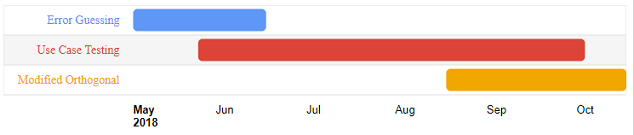
\includegraphics{nis2}
\caption{The planned time period of each testing method}
\end{figure}


\section{Alternative Approaches}

Alternative approaches to this project were considered, but for various reasons these were found to be either inadequate, inferior to the chosen approach, or not suited to the requirements of the project. When the project was initiated, it was decided that broadly scoped, manual testing would form the majority of the tests written for this project. 

While a black-box methodology was chosen for this project, a subset of testing methods had to be chosen, as some methods proved to be unsuitable for the goal of testing a compiler, and the outcomes of other styles were considered to be outweighed by the cost of implementation.
Two other major types of testing were considered, white-box testing, and a more automated testing regime.

\begin{table}
\centering
\begin{threeparttable}
 \caption{A brief comparison of the advantages and disadvantages of testing methodologies considered for this project}
    \begin{tabular}{| l | p{65mm} | p{65mm} |}
    \hline
    \textbf{Testing style} & \textbf{Pros} & \textbf{Cons} \\ \hline
    Black-box &  No knowledge of system required \newline \newline Unbiased view of codebase \newline \newline Tests are relatively uncoupled from system implementation & Practically infinite test state space \newline \newline Lack of knowledge of system may hinder efforts \newline \newline Can lead to large numbers of tests testing the exact same code\\ \hline
    White-box & Knowledge of system may help find bugs \newline \newline Test state space is smaller than black-box \newline \newline Tooling may exist to help testing &  Requires system knowledge \newline \newline Scope of testing can be extremely large \newline \newline Tests may be strongly coupled to implementation  \\ \hline
    Fuzzing & Allows the creation of many tests with little effort \newline \newline Low ongoing time cost  & High initial time cost \newline \newline Difficult to use with compilers \\ \hline
    \end{tabular}
\end{threeparttable}
\end{table}

\subsection{White-box Testing}

White-box, as presented in Section \ref{whitebox}, is a testing methodology that focuses on "test methods that rely on the internal structure of the software" \cite{ostrand}. This means that the author of the tests has to have significant knowledge of the inner workings of the system that they are testing. Major white box testing styles include structured testing \cite{watson}, branch testing, path testing, and statement coverage \cite{ammann} \cite{khan2012}. Some of these techniques could have been useful, but time constraints, the problem domain of a compiler, and the gathered requirements meant that it was felt that a different methodology, namely black-box, would produce better results for this project. 

\subsubsection{Advantages}

One of the main advantages of a white-box testing methodology in regards to this project is that a tester is required to have a good knowledge of the system. This means that the tester may have a good idea of where bugs could be found in the system, as they understand the code, and should therefore understand where testing effort would best be applied. This could be useful in a compiler as knowledge of how the system works at a low level could be helpful in locating bugs.

White-box testing is said to be easy to automate \cite{ammann}, which can be a major advantage, especially when testing a large scale project such as a compiler. Many automated tests could be produced that could provide fairly high branch and statement coverage. 

If statement or branch coverage testing were to be used in a white-box methodology, a clear idea of how "tested" the program is, could be determined. This level of "testedness" could be found by using a simple code coverage tool which would list the percentage of statements and branches covered by unit tests. 

\subsubsection{Disadvantages}

One of the main disadvantages of white-box testing is that a high level of system knowledge is required. This means that before starting testing, the tester will have to spend time familiarising themselves with the system instead of testing. This is especially true in the case of testing a system as complex as a compiler. System knowledge for this project would be difficult to gain in a timely manner, due to the fact that the 42 compiler is a complex system.

Another reason for not using a white-box methodology for this project was that the initial idea of the project is that the compiler would be tested as a whole by creating 42 programs and attempting to run them. There was discussion about the possibility of white-box testing but Dr. Servetto felt it would not be the best path for this project, as it was felt that black-box testing of the system as a whole would be more effective.

Another major problem with white-box testing in terms of this project is that a compiler has a practically infinite input domain. This means that any white-box testing will struggle to fulfil the ideal case of being exhaustive (see Section \ref{whitebox}). White-box testing makes exhaustive unit testing very difficult, especially in regards to path coverage. Due to the extremely large numbers of possible paths, it would be very difficult for path testing to provide any semblance of exhaustiveness in terms of test coverage.

\subsection{Fuzz Testing}

Fuzzing consists of generating random data, called fuzz and using it as input into a program. In the case a of compiler, it would generally consist of generating random programs that could then be attempted to be compiled and run. A prototype, very simple fuzzer, focused on 42 was developed (see the TestIncrementer section below) for this project. It proved to be not very useful, and showed that a "dumb" fuzzer would not be very useful for this project.

Overall it was decided to not pursue fuzzing for this project as existing tools would not have worked very well on the 42 compiler. Specially created "dumb" tools proved they would not be very useful, and a "smart" tool would have taken far too long to create, and would have been significantly out of scope for this project.

\subsubsection{Advantages}

Fuzzing is highly automated once set up, therefore once a fuzzer is initially set up, very little user input would be required, except in the case of dealing with a potential bug the fuzzer has found.

Additionally, due to the fact that fuzzing can be highly automated, fuzzing would produce far more tests than could reasonably be produced manually. If these tests actually managed to test the 42 compiler as a whole (by being syntactically correct 42 programs), fuzzing would be a major help for this project.

\subsubsection{Disadvantages}

Fuzz testing cannot provide a complete picture of the entirety of the program, especially in the case of a compiler. This is because generating random data to test a compiler would probably take the form of generating random strings and trying to compile them as programs. These strings, if randomly generated, are extremely unlikely to be syntactically correct enough to compile, let alone test any interesting behaviour of the 42 language.

Another issue with using fuzzing in this project would be the sourcing of a suitable fuzzer. Most fuzzers are designed to work on C code \cite{afl}. The 42 compiler is coded in Java, and while there are Java fuzzers, they are less advanced and not as effective.

The most effective fuzzer for this project would one that is "smart" enough to be aware of the input structure a file that could be compiled by the 42 compiler. This would probably take the form of a fuzzer that could produce syntactically correct 42 code as an output, and this code could be run and then manually checked if there were some sort of anomaly or error. The creation of this kind of fuzzer would require a significant amount of work, if it is even possible.

\subsubsection{Test Incrementer \label{incrementerSec}}
The 42TestIncrementer \cite{incrementer} is a Python "dumb" fuzzer specifically created for this project. It creates 42 programs by very slightly modifying existing 42 programs. It can be given a .L42 (42's file extension) file, and it will search that file for method declarations. From the given set of method declarations, the incrementer will check through all methods to check if a method takes \textit{Num} (42's arbitrary-precision number class) or an \textit{S} (42's string class) as a method parameter. If a method takes a \textit{Num} or an \textit{S}, the incrementer will modify the parameter in the method call. This modification can either be by set value or random value depending on the way the flags passed to the incrementer.

This program is not particularly advanced, and will only work for method calls that directly have a \textit{Num} or \textit{S} declared in method call. The incrementer had some problems, as there was relatively little time spent developing it, as it was more a proof of concept as opposed to a final polished product. This meant that it is fairly limited; it only works for \textit{Num} and \textit{S} types and does not handle recursion or method overriding very well. It is possible that more time could have been spent on developing the tool, but any more time spent on developing the incrementer would be time that would have had to have been taken away from direct test creation.

The incrementer was a proof of concept and it proved that a "dumb" fuzzer would not be very useful for this project. 42 has arbitrary-precision numbers therefore number overflow was not a risk, and this was the main type of error that the incrementer would have found.

For an example of the 42TestIncrementer see Appendix \ref{incrementerExample} where it is used to slightly modify a program.




 \chapter{Implementation}\label{C:impl}

\section{Overall Testing Strategy}

As discussed in Section \ref{design}, the overall testing methodology employed in this project was a black-box methodology, and multiple different black-box testing methods were used throughout the course of this project.

\subsection{Testing Environment}

Testing took place on two different systems. The first was a Windows 10 system with an Intel i5-4960k and 8GB of RAM, and the other was an Arch Linux system with an Intel i7-6700k and 16GB of RAM. All tests were run on both systems to make sure any bugs found were due to the compiler code, rather than the environment where the testing was taking place. 

\section{Testing Timeline}

In Section \ref{planTiming}, a planned testing timeline was outlined. It proposed that the initial stages of the project would consist of error guessing testing, as it was thought that it would be the most effective method of testing whilst familiarising with the language. The timeline stated that only a short period of time would be spent using this method before use case testing would be used. 

This was not the case in reality. It took longer than expected to become familiarised with the language, especially in regards to some of the more complicated and unique language features. This meant that usage of error guessing lasted longer than planned (two months compared to one month). The usage of use case testing was not majorly impacted by this, as both testing methods were used in parallel.

Another major difference between the plan and the actual implementation is that the usage of modified orthogonal squares was reduced. It was planned that it would be used in parallel with use case testing for around two months at the end of the project. In reality it was only used for approximately two weeks before it was realised that it provided no real benefit. After a discussion with Dr. Servetto, it was realised that due to the practically infinite input domain, there was little proof it was more effective than purely random testing. After this, use of the modified orthogonal squares testing was discontinued.

This meant that majority of testing that took place over the course of this project was use case testing.

\begin{figure}[h]
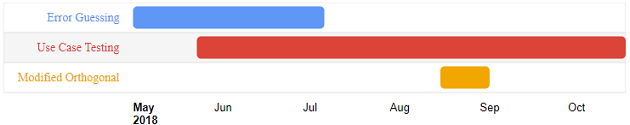
\includegraphics{nis}
\caption{The actual time period of each testing method}
\end{figure}

\section{Techniques Used \label{testMethods}}

\subsection{Error Guessing}

Error guessing, as described in Section \ref{bbtest}, was used over the course of this project. Error guessing was mainly employed at the start of the project as it was a useful testing technique while still familiarising with the language. Error guessing allows the user to take advantage of their previous testing experience. This fact proved useful within this project as research had been done into common compiler bugs. 

Over the course of the project, error guessing found four bugs. The bugs found with error guessing were all bugs in the 42 standard library - Adam's Towel. 

A test developed with error guessing would generally start with a scenario being considered. These scenarios would generally relate to common programming language bugs such as division by zero or invalid method parameters. A program would then be created that used this scenario in some way. This program would then be compiled and run and the result would checked and compared against the expected outcome.

While error guessing and use case testing both used an initial scenario to create the test there were major differences between the two methods. A scenario would be significantly more formal in use case testing as opposed to error guessing. The scenario would also be a lot more carefully followed in use case testing, rather than error guessing.

An example of a test created with error guessing can be seen in Figure \ref{errorguess}. This test was created when the issue of division by zero was considered. A program was written to check what happens when a number is divided by zero. It was decided that the expected outcome of division by zero would be some kind of math error. When the program was created and run, the actual result of one divided by zero was the fraction $\frac{1}{0}$. This test clearly found an error as the actual result ($\frac{1}{0}$) differed from the expected result (an error).

\begin{figure}[h]
	\begin{42listing}
	A: {
		class method divide(Num a, Num b) (
			return a / b
		)
	}
	
	B: {
		Num n = A.divide(a: 1Num, b: 0Num) // We would expect this method call to throw an error.
	}
	\end{42listing}
	\caption{An example of a 42 program created with the error guessing technique \label{errorguess}}
\end{figure}

Another example of a test created with error guessing would include passing different types of parameters to standard library methods than the methods expect. Overall an error guessing test would generally involve writing a 42 program that was not quite syntactically or type correct, and comparing the actual output of the program against what would be expected.



\subsection{Use Case Testing}

Use case testing as described in Section \ref{bbtest} was used in this project. Use case testing was employed throughout the majority of the time of this project and it proved to be extremely useful and effective. One thing to note about the use case testing that was employed in this project was that, compared to the more usual usage of this testing method, the use cases are lower level and focus more on the specific actions that a programmer wants their program to do. The use cases are not fully system orientated, they are still partially user orientated, like use case testing calls for.

A test developed with use case testing would generally follow a set structure. Firstly, a list of actions that would be carried out by a program would be created. The program would then be created using the list of actions as guidelines. This program would then have the actual output compared against the expected output. If the outputs differed, or if an error was thrown, a bug had been identified.

This method of testing allowed for a broad range of programs, and therefore tests, to be created. This is because a use case could be created to target any specific part of the language. For example it is easy to create a use case that tests lists, or a use case that tests inheritance. This allowed for use case testing to test parts of the language that were not covered by other methods of testing. Additionally it allowed for testing of parts of the language that were considered to be more likely to have bugs but would have been difficult to test with other methods. Examples of this include inheritance, which would have been difficult to test with other methods, but was fairly simple with use case testing. 

A scenario of a Cat and Dog class implementing an Animal interface was created. A program was then created, compiled, and run from this scenario. It was then decided to test what would happen if the Dog class was to implement an additional interface. To facilitate this, the scenario and test were simply updated. This was a simple process, and it illustrates the flexibility that use case testing brought to this project.

\begin{figure}[ht]
	\centering
\textbf{Scenario for finding the maximum value in a list of numbers}
	\begin{enumerate}
		\item{Create a list of numbers.}
		\item{Check if the list of numbers is empty.}
		\item{Create a variable that will hold the current maximum value at any point in time.}
		\item{Iterate through the list and check if each number in the list is larger than current maximum. If so, update the current maximum.}
		\item{Return the current maximum value.}
		\item{Assert method result is equal to max list value.}
	\end{enumerate}
	\caption{A list of actions for a program that finds the minimum value in a list of numbers \label{actions}}
	~\\
	\end{figure}

\begin{figure}[ht]
		\begin{42listing}
		A: {
			class method Num max(Nums list) {
				if list.isEmpty() ( // Step 2
					error Undefined"Empty list!"
				)
				
				var Num max = list.val(0Size) // Step 3
				with e in list.vals() ( // Step 4
					if e > max (
						max := e
					)
				)
				return max // Step 5
			}
			
			Nums list = Nums[1Num; 55Num; 0Num; 12Num; 32Num] // Step 1
			X[max(list: list) == 55Num] // Step 6
		}
		\end{42listing}
		\caption{The code for a 42 program that meets the list of actions in \ref{actions}. It is an example of a test created with use case testing \label{figMax}}
\end{figure}

An example of use case testing could be to find the maximum value of a list of numbers and it is shown in Figures \ref{actions} and \ref{figMax}.



\subsection{Orthogonal Squares}

The modified orthogonal squares method (as described in Section \ref{bbtest}) was used during this project. Unfortunately it did not prove to be very effective over the course of this project. It was realised that it did not provide any real benefit over either use case testing or error guessing. After around a week using the method for testing it was realised that it was not producing the desired result (of finding bugs). This led to discussion with Dr. Servetto where it was decided that the method may not have been suitable for testing during this project. It was realised that the 42 compiler is very difficult to test with this method, due to the language itself (e.g. arbitrary-precision numbers, no character class). Additionally Dr. Servetto pointed out that there was no proof the method was any more beneficial than a purely random approach. Due to this it was decided that any testing with this method would be ceased and instead replaced with more use case testing, as it had already proven to be successful. 

The decision to stop using this testing method was backed up by the fact that while it was in use, not a single bug was found with it.



\section{Developed Tools}

\subsection{42TestHelper \label{42TestHelper}}


When a program was written and it was considered to be "interesting" enough to turn it into a test, it would be converted from 42 code to a JUnit \cite{junit} test that would run in the 42 automated test suite, which is written in Java.

\begin{figure}[h]

	\begin{42listing}
	Nums: Collections.vector(of: Num)
	A: {
		primes = Nums[2Num; 11Num; 13Num; 17Num; 19Num]
		var Num initial = 2520Num
		with prime in primes.vals() (
			initial := initial * prime
		)
		return ExitCode.normal()
	}
	\end{42listing}
	\caption{An example of a 42 program \label{42code} that could be turned into a JUnit test}
\end{figure}

\begin{figure}[h]		

\begin{lstlisting}
	@Test
	public void testPrimes() {
		tp("{reuse L42.is/AdamTowel02"
			,"Nums: Collections.vector(of: Num)"
				,"A: {"
			    	,"primes = Nums[2Num; 11Num; 13Num; 17Num; 19Num]"
			    	,"var Num initial = 2520Num"
					,"with prime in primes.vals("
						,"(initial := initial * prime)"
					,")"
			    	,"return ExitCode.normal()"
				,"}"
		,"}");
	}		

\end{lstlisting} 
\caption{The 42 program from Figure \ref{42code} turned into a JUnit test \label{javacode}}
\end{figure}

As seen in Figure \ref{javacode}, turning a 42 program into a test for the 42 test suite requires the creation of a JUnit test that calls a method \textit{tp} that takes a variable number of arguments. Each argument is a string that represents a line of the 42 program. When a test is constructed, the standard JUnit boilerplate is created before the 42 program is turned into a series of strings that are passed as arguments to the \textit{tp} method. This is a fairly time consuming process when done manually, especially when many tests are created at once, or a 42 program is long. During the initial stages of the project, the conversion of 42 programs to JUnit tests was done manually by hand. It was then realised that this could be easily automated as the process required little thinking. A Python tool was created \cite{pytest} that turned 42 code in a JUnit test and could also turn a JUnit test, assuming it contained valid 42 code, into 42 code. A web version of the tool was also created \cite{jstest}. 


This tool greatly sped up the conversion of 42 programs to tests, and allowed the rapid creation of tests, saving significant amounts of time. 

\section{Test Creation Process}

The process of turning a 42 program that had been created with one of the testing methods discussed in Section \ref{testMethods} was fairly straightforward. A program would be created with an expected output, and then the program would be compiled and run. The actual output of the program would then be compared to the expected output.

 If the outputs matched, and no unexpected error was thrown, no bug had been found. In this case, a decision was then made if the program would make an "interesting" test. The "interestingness" of a test was based on how similar the program was to other tests, if it used any unusual language features or syntax, and the result. If a test was deemed to be "interesting" it would then be converted to a JUnit test through the use of the 42TestHelper (see Section \ref{42TestHelper}) and added to the 42 automated test suite.

If the actual and expected output did not match, it was considered likely that a bug had been found. The code would then be minimised, by removing the code which was not necessary to trigger the bug, and it would be checked if the bug had already been found and reported. If not, the bug would be converted into a JUnit test with the 42TestHelper (see Section \ref{42TestHelper}). It would then be added to the 42 automated test suite.

\begin{figure}[h]
\centering
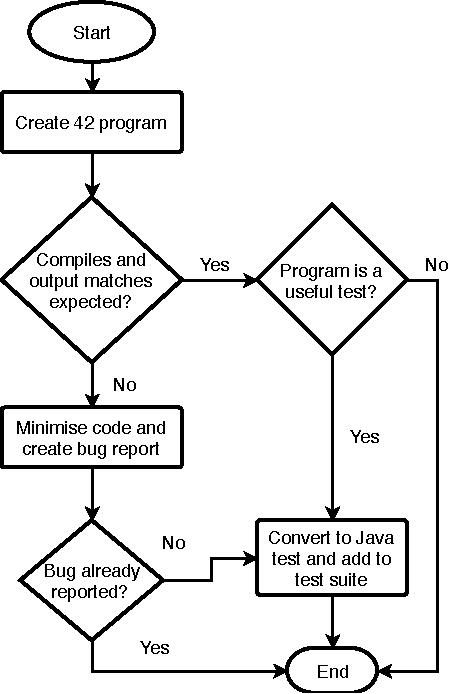
\includegraphics{flowchart}
\caption{A flowchart of creating a standard 42 test}
\end{figure}

  \chapter{Evaluation}\label{C:eval}

\section{Introduction}

Evaluation of this project is difficult as it is impossible to know exactly how many of the bugs that exist in the 42 compiler were found due to this project. It is hard, in practice, to prove that a complex software system is bug-free \cite{EWD:EWD249}. It is possible, but probably not likely, that the vast majority of bugs were found, and also possible, and probably more likely, that this project has barely scratched the surface of the bugs that could be found.

Overall this project has discovered a significant amount of bugs, with 32 previously unidentified bugs being found over the course of the project. The ratio of bugs found to tests written is also quite good, meaning that the effectiveness of each test written was relatively high.


\section{Evaluation Criteria}

It has been decided that this project will be evaluated based on two criteria, the quantity of bugs found, and the nature of the bugs found.

The first criterion was considered the more important as the aim of this project was to find bugs in the 42 compiler, therefore the higher the quantity of bugs found, the more successful the project has been. It was decided that the secondary evaluation criterion would be the categorisation of bugs. Before any bugs were found, eight separate categories that bugs were likely to fall into were decided upon (see Section \ref{cat} for these categories).

\subsection{Quantity of Bugs Found}

Quantity of bugs found is the first and most important criterion. Thirty-two bugs were found over the course of this project, and this is a good outcome for the project, as these bugs were unidentified bugs in the 42 compiler. It is difficult to place this number in context, but one way that has been done is to take the number of programs written over the course of this project, and divide this by the number of tests. This would provide the number of tests written for each bug found over the course of this project, and from this we can also determine the probability of any given test finding a bug. 

\begin{table}[h]
\centering
\begin{threeparttable}
 \caption{The categories and quantity of bugs found}
    \begin{tabular}{| l | c | c |}
    \hline
    \textbf{Category} & \textbf{Quantity} & \textbf{\% of Total Quantity} \\ \hline
    Syntax (too liberal) & 4 & 12.5 \\ \hline
    Syntax (too restrictive) & 4 & 12.5 \\ \hline
    Type system (too liberal) & 1 & 3.1 \\ \hline
    Type system (too restrictive) & 3 & 9.4  \\ \hline
    Metaprogramming (too liberal) & 0 & 0  \\ \hline
    Metaprogramming (too restrictive) & 1  & 3.1 \\ \hline
    Reduction & 6  & 18.8 \\ \hline
    Standard Library Bugs & 7 & 21.9 \\ \hline
    Miscellaneous &  6  & 18.8\\ \hline
    \textbf{Total quantity}	& \textbf{32}  & \textbf{100.1}  \tnote{1} \\ \hline
    \end{tabular}

  \begin{tablenotes}
    \item[1] Percentages do not add up to 100\% due to rounding.
  \end{tablenotes}

\end{threeparttable}


\end{table}

\subsection{Categorisation of Bugs Found \label{cat}}

Before any work beyond language familiarisation was carried out on the project, a set of eight different categories of bugs that were likely to be found was created by Dr. Servetto. This section will provide information on each category. The categorisation of the discovered bugs may not be completely accurate. A reason for this is the fact that some bugs are difficult to categorise, and do not fit nicely into a single category, or they may span over multiple categories. This means that the categorisation of the bugs is not a good tool on which to solely evaluate this project, and the quantity of bugs found therefore must also be taken into account.

\subsubsection{Syntax Bugs}

This category of consists of bugs that are considered to be related to the syntax of 42. This was most common category of bugs found over the course of this project, with eight bugs being found in this category, meaning that 25\% of bugs found were in this category. The large number of bugs in this category could be due to a few different reasons. Firstly, the syntax is extremely easy to test; every time a program is compiled and run the syntax is being tested in some way. Secondly, these bugs are generally easier to find than some other categories, such as the metaprogramming category, especially given the testing methodology employed in this project. 

This category is further split up into two different sub-categories: Syntax (too liberal) and Syntax (too restrictive). Too liberal syntax bugs would be bugs where the syntax is too free, and it allows a user to write 42 code that should not be allowed to compile, as it breaks some sort of syntax rule that should be enforced. Too restrictive syntax bugs are very similar to the too liberal syntax bugs except these bugs mean that a user can write code that meets the language specifications, but the compiler rejects it as syntactically incorrect. 

This category of bugs is generally due to their being a difference between the 42 specification and the implementation of the 42 compiler. This means that a bug falls into this category when during the compilation of the program, an error arises in code that the specification states should compile and run correctly.

\subsubsection{Type System Bugs}

This category consists of bugs that are considered to be related to the type system of 42. This category was the fifth most common category of bugs found over the course of this project, with four bugs being found in this category. With thirty-two bugs found overall, this means that 12.5\% of all bugs found in the course of this project fell into this category. These bugs were not particularly common due to the fact that the 42 type system is theoretically quite sound, and has a strong mathematical basis. 

This category, like the syntax category, can be split up into two sub-categories:  Type system (too liberal) and Type system (too restrictive). Too liberal type system bugs are bugs where the type system is too liberal, and code that is improperly typed is allowed to compile and be run. This code may still display the intended behaviour, depending on the specific bug, but it is still a bug as the compiler should have rejected the code as incorrect. Too restrictive type system bugs are where the type system is too restrictive and code that should have compiled and run correctly does not.

Type system bugs can present a major problem, especially when the type system is too liberal. In this case, code that should be rejected by the type system is accepted and this can lead to major problems when the program runs. When the type system is too restrictive a programmer may be forced to change the way their code works, even though according to the 42 specification it is correct.

The cause of this category of bugs is generally due to some kind of error in the implementation of the 42 compiler, or in rare cases, a difference between the 42 specification and implementation.

\subsubsection{Metaprogramming Bugs \label{meta}}

This category consists of bugs that are considered to be related to the metaprogramming features of 42. This category was the least common category of bugs found over the course of this project, with only one bug being found in this category. With thirty-two bugs found overall, this means that 3.1\% of all bugs found in the course of this project fell into this category. The lack of bugs found in this category probably stems from the lack of metaprogramming testing done for this project. Far fewer tests focused on this category of bugs when compared to the other categories of bugs such as syntax or type system bugs. This was primarily due to a personal lack of knowledge of metaprogamming beyond the basics. Research was done into metaprogramming but it was difficult to gain the knowledge required to thoroughly test the metaprogramming features whilst juggling the other demands of this project. It is known that metaprogramming bugs do exist in the project, as Dr. Servetto has found some examples during his own research.

\subsubsection{Reduction Bugs}

This category includes bugs that are related to the reduction of 42 programs. This category was the third most common category of bugs found over the course of this project, with six bugs being found in this category. This means that 18.8\% of bugs found over the course of this project fell into this category. These bugs were fairly common as program reduction plays a major part in the 42 compilation process, and therefore any program that was compiled and run over the course of this project could have potentially found a bug that fell into this category. 

Reduction bugs are when there is a problem in the conversion process of 42 code into Java bytecode or through an error with javac. These bugs therefore generally take the form of the outputted compiled code's behaviour differing from the expected behaviour of the 42 program that was compiled.

\subsubsection{Standard Library Bugs}

This category consists of bugs in the 42 standard library, Adam's Towel. This category was the second most common category with seven bugs, or 21.9\% of the total found falling into this category.

Adam's Towel provides practically all the basic functionality of 42, apart from base language features like classes. This means that using any language features such as the number or string classes will test the standard library, therefore it is not surprising that finding bugs in this category was common. The bugs in this category took on a wide range of guises due the expansiveness of the standard library.

\subsubsection{Miscellaneous Bugs}

This category of bugs includes all the bugs that did not fit into any of the other previously discussed categories. This category was one of the more common categories of bugs found over the course of this project, with six bugs being found in this category. This means that 18.8\% of bugs found over the course of this project fell into this category. A reason for this is that any bug that did not fit nicely and cleanly into any other category was placed in this one. 



\section{Testing Method}

Overall, use case testing proved to be the most effective testing method used during this project. Use case tests identified twenty-five bugs (78\% of the total bugs) out of thirty-five bugs. This was probably due to a combination of this testing method being used for the majority of the tests, and the flexibility of the testing method.

Error guessing was the second most effective method of testing, with seven bugs found with this method (22\% of the total bugs). More bugs were found with this method than expected, primarily because it was used for longer than was initially planned.

Orthogonal squares was the least effective method of testing with no bugs being identified with this method. This is partially because, due to the lack of effectiveness, the use of this method was discontinued.

\begin{figure}[h]
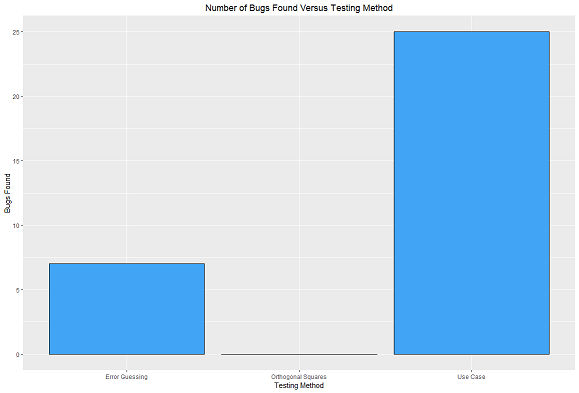
\includegraphics{bugsvmeth}
\caption{A bar graph showing how many bugs each testing method found \label{graph}}
\end{figure}


\section{Overall Evaluation}



\subsection{Quantity Calculations}

Over the course of this project many programs were written and 246 programs were kept, either by being turned into automated tests, or being saved as they were interesting in some way. This is not truly reflective of the number of programs written over the course of this project, because quite often, tests were very similar to previously written tests. This led to the belief that there was not much value in saving them. Only tests that found a bug, or were considered to be unique or interesting were saved. In hindsight, this was a flaw in the project design, as it made it harder to evaluate the overall success of the project. Keeping all the programs and therefore having an accurate number of the tests written would have been helpful for the evaluation.

 This means that any calculations made in regards to the probability of a bug being found per test are potentially flawed, but they still can have some value, especially if a estimation on the total number of programs written is made.

A conservative estimate of the total number of programs written over the course of this project would be around 2,500. This number could be much higher and this estimate is a lower bound that will be used for calculations in the next section. However many of these programs were only slightly different, such as a method parameter being slightly tweaked. There were not 2,500 wholly unique programs created.

\subsubsection{Probability of Finding a Bug}

A useful evaluation metric for this project is the effectiveness of the tests that were written. A good way of measuring the effectiveness of the tests written is calculating how many tests were required to find a single bug. 

If the number of tests written is taken as 246, we can divide this number by the number of bugs found (32), giving an equation of $ 246 / 32 $, which gives an answer of 7.69 tests written for each bug found. This is an low number of tests per bug found, and is an unrealistic representation of the effectiveness of the testing carried out over the course of this project. This is because, as mentioned previously, unfortunately not all the programs that were written were saved, and the number of programs written was not accurately recorded. With the previous estimate of written programs being around 2,500, we can do $ 2500 / 32 $, which gives an answer of 78.13 tests written for each bug found. This is a much more reasonable number of tests when compared to the previous answer of 7.69 tests written per bug found. It is still a low number of tests per bug found, especially when compared to more established languages where thousands of programs can be written without finding a single bug. The reciprocal of the number of tests written per bug found can be taken, and this will give the probability of any given test written over the course of this project finding a bug.

~\\
If we take the number of tests written as 246 we get
\[ \dfrac{1}{246 / 32} \]
\[ = 0.13 \]
Or a probability of $p = 0.13$ of any given test finding a bug.

~\\
If we take the number of tests written as 2,500 we get
\[ \dfrac{1}{2500 / 32} \]
\[ = 0.0128 \]
Or a probability of $p = 0.0128$ of any given test finding a bug.

~\\


\subsection{Bugs Found Over Time}

Over the course of this project, as time went on, the number of bugs found decreased (see Figure \ref{graph}). This could suggest that a significant portion of the bugs in the compiler have been found over the course of this project, as less were found as time went on. However this claim should be approached cautiously, as correlation does not imply causation, but a trend can be seen in terms of the number of bugs found over time. 
\begin{figure}[h]
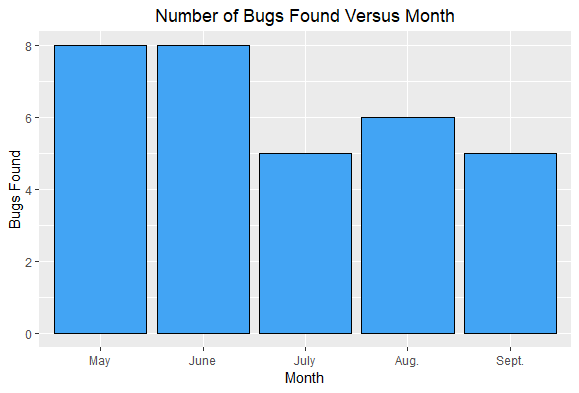
\includegraphics{bugsvsmonth}
\caption{A bar graph showing how many bugs were found per month \label{graph}}
\end{figure}
Alternate reasons for the decreasing number of bugs found could involve changes in the testing method used, or the number of tests written. Overall, this data shows that the number of bugs found over time decreased, but caution should be taken when drawing any conclusions from this data alone.


\section{Summary of Evaluation}

In order to gain an accurate and fair evaluation of this project, the two evaluation criteria previously mentioned, quantity of bugs, and categorisation of bugs, have been used in conjunction. The overall quantity of bugs found was thirty-two, which is a large number of bugs to find in a compiler, especially when considering the fact that they were previously unknown bugs. 

This number can be put in context by taking into account how many tests were written to identify these bugs over the course of this project. 246 programs were recorded as have being written, but not all programs were recorded, and at a conservative estimate, 2,500 tests were written of the course of this project. All evaluation conclusions based off 246 tests will be severely flawed and not accurately reflect the effectiveness of the testing carried out. Therefore the figure of 2,500 programs written will be used for evaluation purposes. Using this figure, 78.13 tests were written for each bug found. This is a very good ratio, and clearly shows that the testing carried out was effective.

The large number of syntax, reduction, and type system bugs found show that the testing carried over the course of this project was quite effective in some areas, but the lack of bugs found in other areas such as metaprogramming shows that there were weak points in the testing.

Overall, finding thirty-two bugs, and finding a bug every seventy-eight tests shows that the testing carried out for this project was effective and well targeted. Finding bugs was the main goal of this project, therefore it can be stated that this project was, on the whole, successful.

 \chapter{Conclusions and Future Work}\label{C:concl}
 
\section{Future Work}

The work undertaken over the course of this project has found a significant number of bugs in the 42 compiler, but it is evident that there is further work that could be carried out to follow on from this project, and it could take the lessons learnt and apply them.

 \subsection{Java to 42 Transpiler \label{trans}}

Linus's Law states that "given enough eyeballs, all bugs are shallow" \cite{cathedral}. This law shows us that the more a program is used, the more bugs are discovered in the program \cite{wang}. This means that more use of the 42 compiler would probably mean the discovery of more bugs, and a good way to use the 42 compiler more is to have a large number of programs to compile and run. A possible way of getting 42 programs could be to create a transpiler with 42 as the target language.

A transpiler, also known as a source-to-source compiler, is a tool that takes source code written in a programming language and produces equivalent code in another language \cite{scotch}. The main difference between a compiler and a transpiler is that a compiler converts high-level source code to low-level instructions that can then be run on some target system \cite{simple}. A transpiler takes source code written in a programming language and converts it to equivalent code in another language that has a similar level of abstraction, and this means that the output code of a transpiler is generally still human readable \cite{scotch}.

A good avenue for future work could be the creation of a transpiler that targeted 42 from another high-level language. 

This project has relied on the creation of 42 programs which were then compiled and run to find bugs, and it has been quite successful, especially given the relatively small number of programs written (around 2,500 programs). A logical continuation of this project could be to continue to create 42 programs and attempt to run and compile them, but programs would still be created relatively slowly. Automatic creation of 42 programs is an additional option, but it would be difficult to create syntactically correct 42 code without the creation of a specific tool that would require large amounts of work and expertise. A potential solution to the lack of 42 programs is converting source code from other languages to 42 source code. The 42 code would then be compiled and run, and the behaviour would be checked against the original code for bugs. If the behaviour or output differs, further investigation would be required to check if the output differs due to a bug in the 42 compiler. 

The development of a 42 transpiler would present some issues. While it would be helpful in the creation of 42 tests, since it would be converting another high-level language to 42, it would mean that some parts of the 42 language would not be tested such as the metaprogramming features or parts of the type system. This is because there is unlikely to be code that would transpiled into 42 metaprogramming, and advanced parts of the type system would be unlikely to be tested. Overall, a transpiler would not produce code that tests the unique or ``special'' parts of the 42 language. 

A reasonable choice for a source language for the transpiler would be Java. This is due to two main reasons; firstly, Java is a commonly used language with a large number of programs written in it, which would give a large pool of programs which could be transpiled to 42 programs. Secondly, transpilation of Java code to another high level language is not a new problem, and examples include J2Eif (Java to Eiffel) \cite{Java2ef} and Google Web Toolkit (Java to JavaScript) \cite{GWT}.


\subsection{Model Checking}

As seen in Section \ref{meta}, very few bugs were found in the metaprogramming system of 42. This means that future work could be prioritised in this area, especially due to the fact that the 42 transpiler as suggested in Section \ref{trans} would not test the 42 metaprogramming features. 

A suggested solution would be to use some sort of model checking to model all outcomes of metaprogramming in a given program. A tool could be created that would take a 42 program with multiple classes, and then all metaprogramming operators (adding, extending, etc.) could be applied over the set of methods. This would allow for fairly easy exhaustive testing of the 42 metaprogramming features, and it could be automated. It would hopefully provide much needed testing of the metaprogramming features of 42, which were not thoroughly tested by this project.

\section{Conclusion}

The goal of this project was to find bugs in the 42 compiler through creating short programs to find corner cases of the 42 implementation. A black-box testing methodology was used for this project, and numerous tests were created with three different black-box testing methods and a tool created to turn programs written in 42 into JUnit tests. The testing mainly focused on use case testing to create tests for this project, with error guessing making up the majority of the remainder of tests written. A planned orthogonal squares method did not work as well as expected and was therefore discontinued.

The testing over the course of the project tests identified thirty-two previously unknown bugs in the 42 compiler. In terms of testing methods, 78\% of bugs were found with use case testing, and 22\% were found with error guessing. This means that use case testing was the most effective and important method of testing employed during this project.

It is estimated that at least 2,500 tests were written over the course of this project. With thirty-two bugs found, on average, it took seventy-eight tests to find each bug. This gives a probability of 1.28\% of any given test finding a bug in the 42 compiler, which shows the testing methods were effective, especially in the case of testing a compiler.

The bugs that were found were split into nine different categories depending on the nature of the bug. Categories included the syntax of the language, the type system, the metaprogramming features, reduction to Java bytecode, standard library bugs, and a miscellaneous category. The most common category of bugs found were syntax bugs followed by standard library bugs, and then reduction and miscellaneous bugs, and this shows that the testing was either particularly effective in these areas, or there were more unidentified bugs in these areas. There was only a single bug found in the metaprogramming category, and this was primarily due to a lack of testing targeting the 42 metaprogramming features rather than a lack of bugs in this area.

Overall the project was successful due to the quantity of bugs found, and the effectiveness of the tests created in terms of the quantity of tests written to bugs found. However the lack of bugs found in the metaprogamming features should be noted, as this showed that the testing was less effective in this area, and future work could be focused more heavily into this area of the compiler.

\begin{appendices}

\chapter{42TestIncrementer Example \label{incrementerExample}}

\begin{figure}[h]
\begin{42listing}
reuse L42.is/AdamTowel02
A: {
	class method incr(Num that) (return that + 1Num)
	class method str(S that) (return that + S"bar")
}
B: {
	Debug(A.incr(1Num))
	Debug(A.str(S"foo"))
	return ExitCode.normal()
}
\end{42listing}
\caption{A 42 program that is a good candidate for the 42TestIncrementer \label{42incr}}
\end{figure}

\begin{figure}[h]
\begin{42listing}
reuse L42.is/AdamTowel02
A: {
	class method incr(Num that) (return that + 1Num)
	class method str(S that) (return that + S"bar")
}

B: {
	Debug(A.incr(13Num))
	Debug(A.str(S"fooTWo"))
	return ExitCode.normal()
}
\end{42listing}
\caption{The 42 program from Figure \ref{42incr} that has been run through the 42TestIncrementer \label{incered}}
\end{figure}


\chapter{Sample bug report}

\textbf{VectorBlankVariable.L42}

\begin{42listing}
	reuse L42.is/AdemTowel02
	CacheAdamTowel02:Load.cacheTowel()

	Nums : Collections.vector(of: Num)
	Main: {
		Nums arr = Nums[_;_;_]
	}
\end{42listing}

~\\
\textbf{Expected behaviour}: Some sort of 42 error stating that variable "\_" is not in scope or cannot be found.

~\\
\textbf{Actual behaviour}: java.lang.NullPointerException
~\\
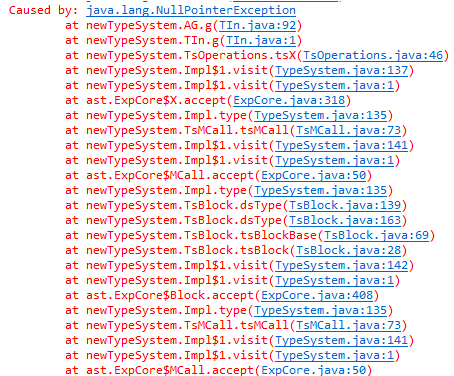
\includegraphics{bugReport}

\end{appendices}


%%%%%%%%%%%%%%%%%%%%%%%%%%%%%%%%%%%%%%%%%%%%%%%%%%%%%%%





\backmatter

%%%%%%%%%%%%%%%%%%%%%%%%%%%%%%%%%%%%%%%%%%%%%%%%%%%%%%%


\bibliographystyle{ieeetr}
%\bibliographystyle{acm}
\bibliography{bibliography}


\end{document}
